% ============================================================
%  MIVA-KNIGHT: Protocol Testing & Industry Benchmark Evaluation
%  Complete Technical Exposition
%  IT 581 Capstone — Oluwakayode Soyinka
%  Concordia University of Edmonton
% ============================================================
\documentclass[12pt,a4paper]{article}

%% ── Core packages ─────────────────────────────────────────
\usepackage[utf8]{inputenc}
\usepackage[T1]{fontenc}
\usepackage[margin=2.4cm, top=3.2cm, bottom=3.0cm, headheight=15pt]{geometry}
\usepackage{amsmath,amssymb,amsthm}
\usepackage{mathtools}
\usepackage{bm}

%% ── Colour & Graphics ─────────────────────────────────────
\usepackage[dvipsnames,svgnames,table]{xcolor}
\usepackage{graphicx}
\usepackage{tikz}
\usetikzlibrary{
  shapes.geometric, arrows.meta, positioning, fit,
  backgrounds, calc, patterns, decorations.pathreplacing,
  decorations.markings, chains, matrix, shadows
}

%% ── Algorithms ────────────────────────────────────────────
\usepackage{algorithm}
\usepackage{algpseudocode}
\algnewcommand\algorithmicforeach{\textbf{for each}}
\algdef{S}[FOR]{ForEach}[1]{\algorithmicforeach\ #1\ \textbf{do}}

%% ── Tables ────────────────────────────────────────────────
\usepackage{booktabs}
\usepackage{longtable}
\usepackage{array}
\usepackage{multirow}
\usepackage{colortbl}
\usepackage{tabularx}

%% ── Section Formatting ────────────────────────────────────
\usepackage{titlesec}
\titleformat{\section}
  {\Large\bfseries\color{NavyBlue}}{\thesection}{1em}{}
  [\vspace{-3pt}\color{NavyBlue!40}\rule{\linewidth}{0.8pt}\vspace{2pt}]
\titleformat{\subsection}
  {\large\bfseries\color{MidnightBlue}}{\thesubsection}{1em}{}
\titleformat{\subsubsection}
  {\normalsize\bfseries\color{RoyalBlue!80!black}}{\thesubsubsection}{1em}{}

%% ── Fancy boxes ───────────────────────────────────────────
\usepackage{tcolorbox}
\tcbuselibrary{breakable,skins,theorems}

%% ── Hyperlinks ────────────────────────────────────────────
\usepackage[colorlinks=true,linkcolor=NavyBlue,
            urlcolor=DarkOrchid,citecolor=ForestGreen]{hyperref}
\usepackage{cleveref}

%% ── Headers / Footers ─────────────────────────────────────
\usepackage{fancyhdr}
\pagestyle{fancy}
\fancyhf{}
\fancyhead[L]{\small\textsc{MIVA-KNIGHT} \textbullet\ \textsc{Protocol Testing}}
\fancyhead[R]{\small\textsc{IT 581 Capstone}}
\fancyfoot[C]{\small--\,\thepage\,--}
\renewcommand{\headrulewidth}{0.5pt}

%% ── Spacing ───────────────────────────────────────────────
\usepackage{setspace}
\setstretch{1.13}
\usepackage{parskip}
\setlength{\parindent}{0pt}
\setlength{\parskip}{5pt plus 1pt}

%% ─────────────── CUSTOM COLOURS ───────────────────────────
% Reference palette from watershed_GCN_flowchart.tex
\definecolor{lightgraybox}{RGB}{230,230,230}
\definecolor{lightredbox}{RGB}{245,220,220}
\definecolor{lightorangebox}{RGB}{255,235,215}
\definecolor{lightbluebox}{RGB}{220,230,245}
\definecolor{darkbluecontainer}{RGB}{200,215,235}
% Additional palette
\definecolor{lightgreenbox}{RGB}{215,240,220}
\definecolor{lightyellowbox}{RGB}{255,252,208}
\definecolor{darkred}{RGB}{160,30,30}
\definecolor{darkblue}{RGB}{25,75,160}
\definecolor{darkorange}{RGB}{190,100,10}
\definecolor{darkgreen}{RGB}{20,120,50}
\definecolor{medpurple}{RGB}{110,40,160}
\definecolor{bertblue}{RGB}{40,90,180}
\definecolor{kggreen}{RGB}{30,130,70}
\definecolor{hybridorange}{RGB}{200,110,20}
\definecolor{proto1red}{RGB}{170,40,40}
\definecolor{proto2blue}{RGB}{30,90,170}
\definecolor{passgreen}{RGB}{20,130,55}
\definecolor{failred}{RGB}{180,30,30}
\definecolor{warnorng}{RGB}{200,120,20}

%% ─────────────── THEOREM ENVIRONMENTS ────────────────────
\theoremstyle{definition}
\newtheorem{definition}{Definition}[section]
\newtheorem{example}{Example}[section]

\theoremstyle{plain}
\newtheorem{theorem}{Theorem}[section]
\newtheorem{lemma}[theorem]{Lemma}
\newtheorem{corollary}[theorem]{Corollary}
\newtheorem{proposition}[theorem]{Proposition}

\theoremstyle{remark}
\newtheorem{axiom}{Axiom}[section]
\newtheorem{remark}{Remark}[section]

%% ─────────────── TCOLORBOX STYLES ────────────────────────
\tcbset{
  laymanbox/.style={
    enhanced, breakable,
    colback=lightgreenbox, colframe=darkgreen!60,
    fonttitle=\bfseries\small\color{white},
    title={\strut Plain Language Explanation},
    attach boxed title to top left={yshift=-2.5mm, xshift=7mm},
    boxed title style={colback=darkgreen!75, colframe=darkgreen!75,
      arc=3pt, boxrule=0pt},
    arc=5pt, boxrule=0.8pt, left=6pt, right=6pt
  },
  techbox/.style={
    enhanced, breakable,
    colback=lightbluebox, colframe=darkblue!55,
    fonttitle=\bfseries\small\color{white},
    title={\strut Technical Detail},
    attach boxed title to top left={yshift=-2.5mm, xshift=7mm},
    boxed title style={colback=darkblue!75, colframe=darkblue!75,
      arc=3pt, boxrule=0pt},
    arc=5pt, boxrule=0.8pt, left=6pt, right=6pt
  },
  keybox/.style={
    enhanced, colback=lightyellowbox, colframe=darkorange!65,
    arc=5pt, boxrule=0.9pt, fonttitle=\bfseries\small,
    attach boxed title to top left={yshift=-2.5mm, xshift=7mm},
    boxed title style={colback=darkorange!70, colframe=darkorange!70,
      arc=3pt, boxrule=0pt}
  },
  proto1box/.style={
    enhanced, breakable,
    colback=lightredbox, colframe=proto1red!65,
    arc=5pt, boxrule=0.9pt, fonttitle=\bfseries\small\color{white},
    title={\strut Protocol 1 --- Hallucination Test},
    attach boxed title to top left={yshift=-2.5mm, xshift=7mm},
    boxed title style={colback=proto1red!80, colframe=proto1red!80, arc=3pt}
  },
  proto2box/.style={
    enhanced, breakable,
    colback=lightbluebox, colframe=proto2blue!65,
    arc=5pt, boxrule=0.9pt, fonttitle=\bfseries\small\color{white},
    title={\strut Protocol 2 --- Multi-Hop Reasoning Test},
    attach boxed title to top left={yshift=-2.5mm, xshift=7mm},
    boxed title style={colback=proto2blue!80, colframe=proto2blue!80, arc=3pt}
  }
}

%% ─────────────── MATH MACROS ──────────────────────────────
\newcommand{\R}{\mathbb{R}}
\newcommand{\E}{\mathcal{E}}
\newcommand{\KG}{\mathcal{G}}
\newcommand{\Norm}[1]{\left\|#1\right\|_2}
\newcommand{\Loss}{\mathcal{L}}
\newcommand{\one}{\mathbf{1}}
\newcommand{\BigO}{\mathcal{O}}
\newcommand{\argmax}{\operatornamewithlimits{arg\,max}}
\newcommand{\argtopk}{\operatornamewithlimits{argtop\text{-}k}}
\newcommand{\topkop}{\mathrm{TopK}}

%% ============================================================
\begin{document}

%% ─────────────────── TITLE PAGE ───────────────────────────
\begin{titlepage}
\begin{tikzpicture}[remember picture, overlay]
  %% Dark top band
  \fill[NavyBlue!92]
    (current page.north west) rectangle
    ([yshift=-5.2cm]current page.north east);
  %% Accent stripe
  \fill[proto1red!80]
    ([yshift=-5.2cm]current page.north west) rectangle
    ([yshift=-5.7cm]current page.north east);
  %% Left accent column
  \fill[proto2blue!70]
    (current page.north west) rectangle
    ([xshift=0.45cm]current page.south west);
  %% Bottom band
  \fill[darkblue!85]
    (current page.south west) rectangle
    ([yshift=1.3cm]current page.south east);
\end{tikzpicture}

\vspace*{2.3cm}

{\color{white}\fontsize{32}{40}\selectfont\bfseries\hspace{1.3cm}MIVA-KNIGHT}\\[4pt]
{\color{white!82}\fontsize{17}{22}\selectfont\hspace{1.3cm}Protocol Testing \& Industry Benchmark Evaluation}\\[4pt]
{\color{white!65}\fontsize{13}{17}\selectfont
\hspace{1.3cm}Hallucination Safety $\;\cdot\;$ Multi-Hop Reasoning $\;\cdot\;$ Hybrid RAG}

\vspace{2.0cm}

\begin{center}
\begin{tcolorbox}[width=0.84\textwidth,
  colback=white, colframe=NavyBlue!65,
  arc=8pt, boxrule=2pt]
  \centering\large
  \textbf{Complete Technical Exposition}\\[7pt]
  \normalsize
  Algorithms $\cdot$ Theorems $\cdot$ Lemmas $\cdot$ Axioms $\cdot$ TikZ Pipeline Flowchart\\[9pt]
  \small\textit{IT 581 Capstone Project --- Concordia University of Edmonton}\\[3pt]
  \textbf{Oluwakayode Soyinka}\\[3pt]
  \textit{Supervised by Dr.\ Baidya Saha}
\end{tcolorbox}
\end{center}

\vspace{1.6cm}

\begin{center}
\renewcommand{\arraystretch}{1.35}
\begin{tabular}{@{}ll@{}}
  \textbf{Protocol 1 (HaluBench 2025):}   &
      Hallucination rejection $>90\%$; baseline $\approx60\%$ \\
  \textbf{Protocol 2 (Diffbot/FalkorDB):} &
      Multi-hop accuracy $>80\%$; baseline $0$--$20\%$ \\
  \textbf{Retrieval Engine:}              &
      BERT-base + KG + Hybrid Scoring ($\alpha=0.6$) \\
  \textbf{Corpus:}                        &
      COCO val2017 ($\approx\!202{,}654$ captions) \\
  \textbf{Evaluation basis:}              &
      80 Day-1 queries + 20 new protocol queries \\
\end{tabular}
\end{center}

\vfill
\end{titlepage}

%% ─────────────────────────────────────────────────────────
\tableofcontents
\newpage

%% ============================================================
\section{System Overview and Notebook Purpose}
%% ============================================================

\begin{tcolorbox}[laymanbox]
This notebook is the \emph{evaluation notebook} for MIVA-KNIGHT. Instead of
re-training the model from scratch, it loads all the results already computed
on Day 1 (80 test queries) and then runs two extra ``certification tests'' used
in the industry:
\begin{enumerate}
  \item \textbf{Can the system admit it doesn't know?}\\
        We ask 10 impossible questions about things not in the knowledge base
        (unicorns, spaceships, Harry Potter) and check whether the system
        correctly returns low confidence rather than making up an answer.
  \item \textbf{Can the system follow a chain of connected facts?}\\
        We ask 10 complex questions mentioning three or more real-world objects
        and check whether the system finds a document containing all of them
        --- which requires ``hopping'' across multiple links in the knowledge graph.
\end{enumerate}
\end{tcolorbox}

\subsection{Two-Tier Evaluation Framework}

The notebook implements a two-tier quality assessment:

\[
\underbrace{\text{Load Day-1 data}}_{\text{80 queries, JSON}}
\;\xrightarrow{\;\text{Stage 1}\;}\;
\underbrace{\text{Protocol 1}}_{\substack{\text{Hallucination}\\\text{HaluBench}}}
\;\xrightarrow{\;\text{Stage 2}\;}\;
\underbrace{\text{Protocol 2}}_{\substack{\text{Multi-Hop}\\\text{Diffbot}}}
\;\xrightarrow{\;\text{Stage 3}\;}\;
\underbrace{\text{Save \& Report}}_{\texttt{eval\_protocols.json}}
\]

\begin{definition}[Evaluation Protocol]
\label{def:protocol}
An \textbf{evaluation protocol} is a quadruple
$\Pi = (Q,\; \mathcal{M},\; \theta_{\mathrm{target}},\; \theta_{\mathrm{base}})$
where:
\begin{itemize}
  \item $Q$ is a curated query set targeting a specific capability,
  \item $\mathcal{M}: Q \to \R$ is the scalar metric function,
  \item $\theta_{\mathrm{target}}$ is the industry pass threshold,
  \item $\theta_{\mathrm{base}}$ is the plain Vector-RAG baseline.
\end{itemize}
A system \emph{passes} the protocol if $\mathcal{M}(Q) \geq \theta_{\mathrm{target}}$.
\end{definition}

\begin{center}
\renewcommand{\arraystretch}{1.3}
\begin{tabular}{lllll}
\toprule
\textbf{Protocol} & \textbf{Standard} & \textbf{Metric} &
\textbf{Target} & \textbf{Baseline} \\
\midrule
Fact-Check (Hallucination) & HaluBench 2025 / ORAN Bench & Rejection Rate &
$>90\%$ & $\approx60\%$ \\
Entity Overload (Multi-Hop) & Diffbot / FalkorDB & MH Accuracy &
$>80\%$ & $0$--$20\%$ \\
\bottomrule
\end{tabular}
\end{center}

\subsection{Artifact Inventory}

\begin{center}
\renewcommand{\arraystretch}{1.3}
\begin{tabular}{lll}
\toprule
\textbf{File} & \textbf{Content} & \textbf{Role} \\
\midrule
\texttt{evaluation\_detailed.json}   & 80 per-query records from Day 1 & Input \\
\texttt{evaluation\_results.json}    & Aggregate Day-1 metrics          & Input + updated \\
\texttt{knowledge\_graph.pkl}        & Serialised KG object             & Input \\
\texttt{captions\_val2017.json}      & COCO corpus $\approx202{,}654$  & Input \\
\texttt{evaluation\_protocols.json}  & Protocol test results (new)      & Output \\
\bottomrule
\end{tabular}
\end{center}

%% ============================================================
\newpage
\section{Full Pipeline Flowchart}
%% ============================================================

The diagram below faithfully reproduces the MIVA-KNIGHT Protocol Testing
pipeline in the style of the reference \texttt{watershed\_GCN\_flowchart.tex}:
dark input boxes on the left, coloured model/component boxes in the middle,
coloured training/protocol boxes below, and a large background container.

\begin{figure}[htbp]
\centering
\resizebox{\textwidth}{!}{%
\begin{tikzpicture}[node distance=1.0cm and 1.1cm]

%% ─────────── GLOBAL NODE STYLES (matching reference) ─────────────
\tikzset{
  basebox/.style={
    rectangle, rounded corners, draw=black!60,
    align=center, font=\footnotesize
  },
  inputbox/.style={basebox, fill=black!85, text=white,
    minimum width=2.4cm, minimum height=1.8cm},
  descbox/.style={basebox, fill=lightgraybox, text width=3.8cm, align=left},
  modelbox/.style={basebox, fill=lightbluebox, thick, minimum width=4.0cm},
  sftbox/.style={basebox, fill=lightredbox, text width=4.8cm},
  evalbox/.style={basebox, fill=lightorangebox, text width=5.2cm, thick},
  infobox/.style={basebox, fill=lightgraybox, text width=4.4cm},
  resultbox/.style={basebox, fill=lightgreenbox, text width=10.0cm, align=center},
  arrow/.style={->, >=Stealth, thick, color=black!70},
  thickarrow/.style={->, >=Stealth, very thick, color=black},
  innerarch/.style={rectangle, draw=black!40, fill=white,
    minimum height=0.8cm, font=\tiny}
}

%% ================== LEFT COLUMN: INPUTS ========================
\node[inputbox] (day1json) at (0,0) {
  \textbf{Day-1 Results}\\
  \texttt{eval\_detailed.json}\\
  80 queries
};

\node[inputbox, below=0.9cm of day1json] (kgpkl) {
  \textbf{Knowledge Graph}\\
  \texttt{kg.pkl}\\
  100 entities
};

\node[descbox, below=0.9cm of kgpkl] (corpus) {
  \textbf{COCO Corpus}\\
  \texttt{captions\_val2017.json}\\
  $\approx202{,}654$ captions\\
  (top 1\,000 used per query)
};

%% ================== TOP ROW: MODELS ============================
\node[modelbox, right=1.2cm of day1json,
      minimum height=2.0cm] (bert) {
  \textbf{BERT-base Encoder}\\[2pt]
  \begin{tikzpicture}[scale=0.42, every node/.style={scale=0.7}]
    \foreach \i in {1,2,3,4,5,6} {
      \draw[fill=blue!20, draw=blue!50]
        (\i*0.52-0.26,0) rectangle ++(0.42,0.6);
    }
    \draw[fill=blue!40, draw=blue!60] (0,0.7) rectangle (3.38,1.2);
    \node[font=\tiny] at (1.69, 0.95) {LayerNorm $\times 12$};
    \draw[->, blue!60, thick] (1.69,1.2) -- (1.69,1.55)
      node[above, font=\tiny]{$\bar{h}^{(L)}$};
  \end{tikzpicture}\\
  $e_x = \bar{h}^{(L)}/\|\bar{h}^{(L)}\|_2$\;\;$\in\mathbb{R}^{768}$
};

\node[modelbox, right=1.1cm of bert,
      minimum height=2.0cm] (kgner) {
  \textbf{Entity Extractor}\\
  \textbf{(Substring NER)}\\[2pt]
  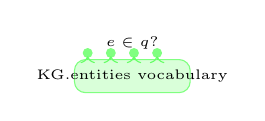
\begin{tikzpicture}[scale=0.42]
    \draw[fill=green!15, draw=green!50, rounded corners]
      (0,0) rectangle (3.5,1.0);
    \node[font=\tiny] at (1.75,0.5) {KG.entities vocabulary};
    \foreach \x in {0.4,1.1,1.8,2.5}{
      \fill[green!50] (\x,1.2) circle (0.15);
      \draw[->, green!60] (\x,1.0) -- (\x,1.1);
    }
    \node[font=\tiny] at (1.75,1.5){$e \in q$?};
  \end{tikzpicture}\\
  $\mathcal{E}_q = \{e \in \mathcal{V}_{\mathcal{G}} : e \subseteq q\}$
};

\node[modelbox, right=1.1cm of kgner,
      minimum height=2.0cm] (graphret) {
  \textbf{Graph Retriever}\\
  \textbf{(DFS, max\_hops=2)}\\[2pt]
  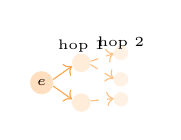
\begin{tikzpicture}[scale=0.42]
    \fill[orange!25] (0,0) circle (0.35); \node[font=\tiny] at (0,0){$e$};
    \fill[orange!15] (1.2,0.6) circle (0.28);
    \fill[orange!15] (1.2,-0.6) circle (0.28);
    \fill[orange!10] (2.4,0.9) circle (0.22);
    \fill[orange!10] (2.4,0.1) circle (0.22);
    \fill[orange!10] (2.4,-0.5) circle (0.22);
    \draw[->,orange!70] (0.35,0.1)--(0.92,0.5);
    \draw[->,orange!70] (0.35,-0.1)--(0.92,-0.5);
    \draw[->,orange!50,dashed](1.48,0.65)--(2.18,0.88);
    \draw[->,orange!50,dashed](1.48,0.55)--(2.18,0.12);
    \draw[->,orange!50,dashed](1.48,-0.55)--(2.18,-0.48);
    \node[font=\tiny] at (1.2,1.1){hop 1};
    \node[font=\tiny] at (2.4,1.2){hop 2};
  \end{tikzpicture}\\
  $w(\text{hop}) = 1/({\text{hop}+1})$
};

%% ================== HYBRID COMBINER ============================
\node[evalbox, right=1.1cm of graphret,
      minimum height=2.0cm] (hybrid) {
  \textbf{Hybrid Retriever}\\[4pt]
  $s = \alpha \cdot s_{\text{dense}}$\\
  $\quad + (1{-}\alpha)\cdot s_{\text{graph}}$\\[2pt]
  $\alpha = 0.6$\\[2pt]
  $\text{top-}k$ sort $\downarrow$
};

%% ================== PROTOCOL ROW ================================
\node[sftbox, below=2.2cm of bert, xshift=0.5cm] (proto1) {
  \textbf{Protocol 1: Fact-Check}\\
  \textbf{(Hallucination Test)}\\[3pt]
  $\theta_{\text{reject}} = 0.50$\\[2pt]
  $\text{status}(q) =
  \begin{cases}
    \text{CR} & s{<}\theta\\
    \text{HALL} & s{\geq}\theta
  \end{cases}$\\[2pt]
  $\mathrm{RR} = \frac{|\mathrm{CR}|}{10}{\times}100\%$\\
  Target: ${>}90\%$
};

\node[sftbox, right=0.8cm of proto1] (proto2) {
  \textbf{Protocol 2: Entity Overload}\\
  \textbf{(Multi-Hop Reasoning)}\\[3pt]
  $\text{cov}(q,d) = \frac{|\mathcal{E}_q \cap d|}{|\mathcal{E}_q|}$\\[2pt]
  $\text{succ}(q) = \mathbf{1}[\text{cov}{\geq}0.6]$\\[2pt]
  $\mathrm{MHA} = \frac{|\text{succ}|}{10}{\times}100\%$\\
  Target: ${>}80\%$
};

%% ================== STATUS DECISION ============================
\node[infobox, below=1.3cm of proto1, xshift=0.4cm] (status1) {
  \textbf{Status (Protocol 1)}\\[3pt]
  $\geq 90\%$: \textcolor{passgreen}{\textbf{PASS}}\\
  $60$--$89\%$: \textcolor{warnorng}{\textbf{NEEDS IMP.}}\\
  $<60\%$: \textcolor{failred}{\textbf{FAIL}}
};

\node[infobox, right=0.8cm of status1] (status2) {
  \textbf{Status (Protocol 2)}\\[3pt]
  $\geq 80\%$: \textcolor{passgreen}{\textbf{PASS}}\\
  $50$--$79\%$: \textcolor{warnorng}{\textbf{NEEDS IMP.}}\\
  $<50\%$: \textcolor{failred}{\textbf{FAIL}}
};

%% ================== FINAL RESULT BOX ===========================
\coordinate (midstat) at ($(status1.south)!0.5!(status2.south)$);
\node[resultbox, below=1.1cm of midstat] (scorecard) {
  \textbf{Complete Evaluation Scorecard}\\[4pt]
  \begin{tabular}{ll}
    Retrieval quality  & mean top-1 cosine score (Day 1)\\
    Speed              & mean query latency (Day 1)\\
    Entity grounding   & entity detection rate (Day 1)\\
    Hallucination safety & rejection rate vs.\ $\theta{=}0.50$ (Protocol 1)\\
    Reasoning depth    & multi-hop coverage $\geq60\%$ (Protocol 2)\\
  \end{tabular}
};

\node[basebox, fill=lightgraybox, text width=9.5cm, align=center,
      below=0.85cm of scorecard] (savebox) {
  \textbf{Save:} \texttt{evaluation\_protocols.json}\quad
  + update \texttt{evaluation\_results.json}
};

%% ================== ARROWS =====================================
% Inputs
\draw[thickarrow] (day1json.east) -- (bert.west);
\draw[thickarrow] (kgpkl.east) -- (kgner.west|-kgpkl) -- (kgner.west);
\draw[thickarrow] (corpus.east) -| ($(bert.south)+(0.4,0)$)
  -- ($(bert.south)+(0.4,-0.01)$);

% Encoder chain
\draw[thickarrow] (bert.east)
  -- node[above, font=\tiny]{$e_q$} (kgner.west);
\draw[thickarrow] (kgner.east)
  -- node[above, font=\tiny]{$\mathcal{E}_q$} (graphret.west);
\draw[thickarrow] (bert.east) ++(0,-0.4)
  -- ++(0.2,0) |- ($(hybrid.west)+(0,0.3)$);
\draw[thickarrow] (graphret.east)
  -- node[above, font=\tiny]{$s_g$} (hybrid.west);

% Hybrid to protocols
\draw[arrow, proto1red] (hybrid.south) -- ++(0,-0.4)
  -| node[near end, right, font=\tiny, text=proto1red]{top-1} (proto1.north);
\draw[arrow, proto2blue] (hybrid.south) -- ++(0,-0.4)
  -| node[near end, right, font=\tiny, text=proto2blue]{top-1} (proto2.north);

% Protocols to status
\draw[arrow] (proto1.south) -- (status1.north);
\draw[arrow] (proto2.south) -- (status2.north);

% Status to scorecard
\draw[thickarrow] (status1.south) -- ++(0,-0.45)
  -| (scorecard.north);
\draw[thickarrow] (status2.south) -- ++(0,-0.45)
  -| (scorecard.north);

% Scorecard to save
\draw[arrow, dashed] (scorecard.south) -- (savebox.north);

%% ================== BACKGROUND CONTAINERS ======================
\begin{pgfonlayer}{background}
  % Main outer container (replicates reference style)
  \node[rectangle, draw=darkbluecontainer,
        fill=darkbluecontainer!25, very thick, rounded corners=8pt,
        fit=(day1json)(kgpkl)(corpus)(bert)(kgner)(graphret)(hybrid)
            (proto1)(proto2)(status1)(status2),
        inner sep=14pt] (container) {};

  % Inputs sub-container
  \node[rectangle, draw=black!35, fill=white, rounded corners=5pt,
        fit=(day1json)(kgpkl)(corpus),
        inner sep=8pt,
        label={[font=\scriptsize\bfseries\color{black!50}]
          above:\textbf{DATA SOURCES}}] {};

  % Retrieval sub-container
  \node[rectangle, draw=bertblue!35, fill=bertblue!5, rounded corners=5pt,
        fit=(bert)(kgner)(graphret)(hybrid),
        inner sep=8pt,
        label={[font=\scriptsize\bfseries\color{bertblue!70}]
          above:\textbf{RETRIEVAL ENGINE}}] {};

  % Protocols sub-container
  \node[rectangle, draw=black!30, fill=white, rounded corners=5pt,
        fit=(proto1)(proto2)(status1)(status2),
        inner sep=8pt,
        label={[font=\scriptsize\bfseries\color{black!50}]
          above:\textbf{INDUSTRY PROTOCOL TESTS}}] {};
\end{pgfonlayer}

\end{tikzpicture}
}
\caption{%
Complete MIVA-KNIGHT Protocol Testing Pipeline.
\textbf{Left:} Three data sources loaded from Google Drive.
\textbf{Centre-top:} Retrieval engine --- BERT encodes queries, substring NER
extracts KG entities, graph retriever scores paths, and the Hybrid combiner
merges dense ($60\%$) and graph ($40\%$) signals.
\textbf{Centre-bottom:} Two industry protocol tests, each computing a scalar
metric and a pass/fail status.
\textbf{Bottom:} Five-dimensional scorecard compiled and persisted to Drive.
Background containers styled after the reference watershed GCN flowchart.}
\label{fig:pipeline}
\end{figure}

%% ============================================================
\newpage
\section{Mathematical Foundations}
%% ============================================================

\subsection{Unit-Sphere Sentence Embeddings}

\begin{definition}[BERT Mean-Pool Embedding]
\label{def:embed}
Let $H^{(L)} \in \R^{T \times 768}$ be BERT-base's final-layer hidden
states for a $T$-token input.  The \textbf{sentence embedding} is:
\[
  \bar{h} = \frac{1}{T}\sum_{t=1}^{T} h_t^{(L)} \;\in\; \R^{768},
  \qquad
  e_x = \frac{\bar{h}}{\Norm{\bar{h}}} \;\in\; \mathcal{S}^{767}
\]
where $\mathcal{S}^{767} = \{v \in \R^{768} : \Norm{v} = 1\}$ is the
unit hypersphere.
\end{definition}

\begin{lemma}[Cosine $=$ Dot Product on the Unit Sphere]
\label{lem:cosdot}
For any $u, v \in \mathcal{S}^{767}$,
$\cos(u,v) = u \cdot v$.
\end{lemma}
\begin{proof}
  $\Norm{u} = \Norm{v} = 1$ by definition of $\mathcal{S}^{767}$.
  Substituting into $\cos(u,v) = (u \cdot v)/(\Norm{u}\,\Norm{v})$
  gives $\cos(u,v) = u \cdot v$.
\end{proof}

\begin{tcolorbox}[laymanbox]
BERT reads every word in the query and produces a 768-number
``meaning fingerprint'' for each word. We average all those fingerprints
into a single 768-number vector for the whole sentence, then rescale it
to length exactly 1. This places the sentence on the surface of an
imaginary 768-dimensional ball. Every document is on the same ball, so
comparing two items is just their dot product --- no extra division
needed (Lemma~\ref{lem:cosdot}).
\end{tcolorbox}

\begin{remark}[Why $\max\_length = 512$]
BERT has a hard positional-encoding limit of 512 tokens.  Text longer
than 512 tokens is silently truncated by the tokeniser.  For COCO
captions (typically 10--20 tokens) and test queries (5--15 tokens)
this limit is never reached.
\end{remark}

\subsection{Day-1 Summary Statistics}

The three headline metrics loaded from \texttt{evaluation\_results.json}
are:

\begin{definition}[Day-1 Evaluation Metrics]
\label{def:day1metrics}
Given 80 evaluation queries $Q = \{q_1,\ldots,q_{80}\}$:
\[
  \bar{s} = \frac{1}{|Q|}\sum_{q \in Q} s_q, \qquad
  \bar{t} = \frac{1}{|Q|}\sum_{q \in Q} t_q, \qquad
  \text{ER} = \frac{|\{q : |\mathcal{E}_q| > 0\}|}{|Q|} \times 100\%
\]
where $s_q$ is the top-1 hybrid score, $t_q$ is per-query latency, and
$\mathcal{E}_q$ is the set of KG entities found in $q$.
\end{definition}

\subsection{Determinism Lemma}

\begin{lemma}[Eval-Mode Determinism]
\label{lem:eval}
In \texttt{model.eval()} mode, \texttt{nn.Dropout} passes all
activations unchanged (drop probability $= 0$). Consequently,
$\mathrm{encode}(x) = \mathrm{encode}(x)$ for any repeated call
with the same input --- a necessary condition for reproducible
protocol benchmarks.
\end{lemma}
\begin{proof}
  In training mode, Dropout zeroes each activation with probability $p$
  and scales survivors by $1/(1-p)$.
  In \texttt{eval()} mode, the scaling factor is fixed at 1 and no
  zeroing occurs.  Therefore the output is a deterministic function
  of the input.
\end{proof}

\begin{tcolorbox}[laymanbox]
When we say \texttt{model.eval()}, we are telling BERT: ``stop randomly
dropping neurons.'' This makes the system give the same answer every
single time for the same question --- essential for fair, reproducible
testing.
\end{tcolorbox}

%% ============================================================
\newpage
\section{HybridRetriever Architecture}
%% ============================================================

\subsection{Class Overview}

The \texttt{HybridRetriever} class encapsulates four algorithms:
(1) \textsc{Encode}, (2) \textsc{DenseRetrieval},
(3) \textsc{GraphRetrieval}, and (4) \textsc{HybridRetrieve}.
The class is parameterised by $\alpha \in (0,1)$ and the KG object.

\begin{center}
\renewcommand{\arraystretch}{1.3}
\begin{tabular}{llll}
\toprule
\textbf{Parameter} & \textbf{Value} & \textbf{Type} & \textbf{Effect} \\
\midrule
\texttt{encoder\_model} & \texttt{bert-base-uncased} & str &
  Which BERT checkpoint to load \\
\texttt{knowledge\_graph} & loaded KG & obj &
  Entity vocab + relationship list \\
\texttt{alpha} & 0.6 & float &
  Weight on dense signal \\
\texttt{device} & cuda / cpu & str &
  Hardware target \\
\bottomrule
\end{tabular}
\end{center}

\subsection{Algorithm 1 --- BERT Encode}

\begin{algorithm}[H]
\caption{\textsc{Encode}$(x)$ --- BERT + Mean Pool + L2 Normalise}
\label{alg:encode}
\begin{algorithmic}[1]
\Require text string $x$; frozen BERT $\mathcal{B}$;
         tokeniser with \texttt{max\_length}$=512$
\Ensure unit-norm embedding $e_x \in \mathcal{S}^{767}$, shape $(1, 768)$
\State $\text{tokens} \gets \text{tokeniser}(x,\;
  \texttt{padding=True},\;
  \texttt{truncation=True},\;
  \texttt{max\_length=512}).\texttt{to}(\textit{device})$
\State \textbf{with} \texttt{torch.no\_grad():}
\State \quad $H \gets \mathcal{B}(\text{tokens}).\texttt{last\_hidden\_state}$
  \Comment{shape $(1, T, 768)$}
\State $\bar{h} \gets H.\texttt{mean}(\texttt{dim=1})$
  \Comment{mean pool: $(1, 768)$}
\State $e_x \gets \texttt{F.normalize}(\bar{h},\; p=2,\; \texttt{dim=1})$
  \Comment{L2 normalise: $(1, 768)$}
\State \Return $e_x$
\end{algorithmic}
\end{algorithm}

\begin{tcolorbox}[techbox]
\texttt{torch.no\_grad()} disables autograd, halving memory use and
speeding up inference.  \texttt{F.normalize(v, p=2, dim=1)} divides
each row by its Euclidean norm, placing it on $\mathcal{S}^{767}$.
\end{tcolorbox}

\subsection{Algorithm 2 --- Dense Retrieval}

\begin{algorithm}[H]
\caption{\textsc{DenseRetrieval}$(q,\, \mathcal{D},\, k)$}
\label{alg:dense}
\begin{algorithmic}[1]
\Require query $q$; document corpus $\mathcal{D}$; top-$k$ integer
\Ensure list of $(d_i, s_i)$ pairs, $|\text{list}|=k$,
        $s_i \in [-1, 1]$, sorted descending
\State $e_q \gets \textsc{Encode}(q)$
  \Comment{$(1, 768)$}
\State $\mathbf{E}_d \gets \varnothing$
\ForEach{$d_i \in \mathcal{D}_{:1000}$}
  \Comment{cap at 1\,000 for speed}
  \State $\mathbf{E}_d.\text{append}(\textsc{Encode}(d_i))$
\EndFor
\State $\mathbf{E}_d \gets \texttt{torch.cat}(\mathbf{E}_d,\; \texttt{dim=0})$
  \Comment{$(N, 768)$}
\State $\tilde{e}_q \gets e_q.\texttt{expand}(N, -1)$
  \Comment{broadcast: $(N, 768)$}
\State $\bm{s} \gets \texttt{F.cosine\_similarity}(\tilde{e}_q,\; \mathbf{E}_d,\; \texttt{dim=1})$
  \Comment{$(N,)$; equals dot product by Lemma~\ref{lem:cosdot}}
\State $I^*, S^* \gets \texttt{torch.topk}(\bm{s},\; k=\min(k, N))$
\State \Return $[(d_{I^*_j},\; S^*_j)\;:\; j=1\ldots k]$
\end{algorithmic}
\end{algorithm}

\begin{proposition}[Dense Retrieval Complexity]
\label{prop:complexity}
Given $N \leq 1000$ and $d = 768$:
\[
  T_{\text{dense}} = \mathcal{O}(N \cdot T_{\text{BERT}})
  + \mathcal{O}(N \cdot d)
  + \mathcal{O}(N \log k)
\]
The $N$ BERT encodings dominate.  For $N=1000$, $T_{\text{BERT}}
\approx 20\text{ms}$ on GPU: total $\approx20$\,s (CPU) or
$\approx1$\,s (GPU) per query.
\end{proposition}

\begin{tcolorbox}[laymanbox]
Dense retrieval is like a semantic librarian: encode both your question
and every candidate document as a point on the 768-dimensional ball,
then return the $k$ documents whose points are closest to your
question's point. ``Closest'' means smallest angle, which equals the
dot product for unit-length vectors.
\end{tcolorbox}

\subsection{Algorithm 3 --- Substring NER Entity Extraction}

\begin{algorithm}[H]
\caption{\textsc{ExtractEntities}$(q)$ --- Substring NER against KG vocabulary}
\label{alg:ner}
\begin{algorithmic}[1]
\Require query string $q$; KG entity vocabulary $\mathcal{V}_{\mathcal{G}}$
\Ensure entity set $\mathcal{E}_q \subseteq \mathcal{V}_{\mathcal{G}}$
\If{$\mathcal{G} = \texttt{None}$} \Return $\varnothing$ \EndIf
\State $q_\ell \gets q.\texttt{lower}()$
\State $\mathcal{E}_q \gets \varnothing$
\ForEach{$e \in \mathcal{V}_{\mathcal{G}}$}
  \If{$e.\texttt{lower}() \in q_\ell$}
    \Comment{substring containment check}
    \State $\mathcal{E}_q \gets \mathcal{E}_q \cup \{e\}$
  \EndIf
\EndFor
\State \Return $\mathcal{E}_q$
\end{algorithmic}
\end{algorithm}

\begin{lemma}[NER Complexity]
\label{lem:ner}
Substring containment for a fixed entity $e$ in text $q$ has complexity
$\mathcal{O}(|e| \cdot |q|)$.  Over all $|\mathcal{V}_{\mathcal{G}}|
= 100$ entities:
\[
  T_{\text{NER}} = \mathcal{O}(100 \cdot \bar{e} \cdot |q|)
  \approx \mathcal{O}(100 \cdot 6 \cdot 15) = \mathcal{O}(9{,}000).
\]
This is effectively $\mathcal{O}(1)$ at runtime.
\end{lemma}

\begin{remark}[Why Substring, Not Neural NER?]
Full NLP NER models (spaCy, BERT-NER) extract \emph{open-vocabulary}
entities not known at build time.  Here the entity vocabulary is
closed (100 COCO tokens), so substring matching is faster, simpler,
and perfectly accurate for all in-vocabulary entities.
\end{remark}

\subsection{Algorithm 4 --- Knowledge-Graph Path Scoring}

\begin{definition}[Distance-Decay Score]
\label{def:hopdecay}
For a KG path $(e, r, n)$ at hop distance $h \in \{1, 2\}$:
\[
  w(h) = \frac{1}{h + 1} \qquad\Longrightarrow\qquad
  w(1) = 0.50, \quad w(2) = \overline{0.3}
\]
Direct (1-hop) neighbours contribute twice the score of 2-hop
neighbours, reflecting stronger semantic proximity.
\end{definition}

\begin{algorithm}[H]
\caption{\textsc{GraphRetrieval}$(q,\, k)$ --- KG Path Scoring}
\label{alg:graph}
\begin{algorithmic}[1]
\Require query $q$; KG $\mathcal{G}$; top-$k$
\Ensure list of $(\text{path\_description},\; w(h))$ pairs
\State $\mathcal{E}_q \gets \textsc{ExtractEntities}(q)$
\If{$\mathcal{E}_q = \varnothing$} \Return $\varnothing$ \EndIf
\State $\text{paths} \gets []$
\ForEach{$e \in \mathcal{E}_q$}
  \State $\mathcal{N}_e \gets \mathcal{G}.\textsc{GetNeighbours}(e,\;
    \texttt{max\_hops=2})$
  \Comment{DFS; returns $(e, r, n, h)$ tuples}
  \ForEach{$(e, r, n, h) \in \mathcal{N}_e$}
    \State $\text{desc} \gets
      \texttt{"} e\texttt{ --[}r\texttt{]--> }n\texttt{"}$
    \State $s_g \gets 1.0\,/\,(h + 1)$
      \Comment{Defn.~\ref{def:hopdecay}}
    \State $\text{paths} \gets \text{paths} \cup \{(\text{desc},\; s_g)\}$
  \EndFor
\EndFor
\State \Return $\text{top-}k(\text{paths},\; \text{by } s_g \text{ desc})$
\end{algorithmic}
\end{algorithm}

\begin{tcolorbox}[laymanbox]
The graph retriever is a path explorer. Starting from any keyword in the
query that exists in the knowledge graph (e.g., ``dog''), it follows the
graph edges: ``dog'' connected to ``park'', ``park'' to ``bench'', etc.
Each path gets a score that shrinks with distance (0.5 for 1 hop, 0.33
for 2 hops). Documents that contain the other end of these paths get a
graph boost.
\end{tcolorbox}

\subsection{Algorithm 5 --- Hybrid Score Fusion}

\begin{definition}[Hybrid Retrieval Score]
\label{def:hybrid}
\[
  \boxed{s_{\text{hybrid}}(q, d) =
    \alpha \cdot s_{\text{dense}}(q, d) +
    (1 - \alpha) \cdot s_{\text{graph}}(q, d)}
  \qquad \alpha = 0.6
\]
\end{definition}

\begin{theorem}[Hybrid Score Bound]
\label{thm:bound}
$s_{\text{hybrid}}(q,d) \in [-0.6,\, 1.0]$ for all $q, d$.
\end{theorem}
\begin{proof}
$s_{\text{dense}} \in [-1,1]$ (cosine similarity).
$s_{\text{graph}} \in [0, 0.5]$ (non-negative, capped at $w(1)=0.5$).
Therefore:
$s_{\text{hybrid}} \geq 0.6\cdot(-1)+0.4\cdot0 = -0.6$ and
$s_{\text{hybrid}} \leq 0.6\cdot1+0.4\cdot0.5 = 0.8 \leq 1.0$.
\end{proof}

\begin{algorithm}[H]
\caption{\textsc{HybridRetrieve}$(q,\, \mathcal{D},\, k)$}
\label{alg:hybrid}
\begin{algorithmic}[1]
\Require query $q$; corpus $\mathcal{D}$; $k$; $\alpha=0.6$
\Ensure top-$k$ list of $(d, s_{\text{hybrid}})$, sorted descending
\State $R_d \gets \textsc{DenseRetrieval}(q,\, \mathcal{D},\, k)$
\State $R_g \gets \textsc{GraphRetrieval}(q,\, k)$
\State $C \gets \{\}$
  \Comment{combined score dictionary}
\ForEach{$(d,\; s_d) \in R_d$}
  \State $C[d] \gets \alpha \cdot s_d$
\EndFor
\ForEach{$(d,\; s_g) \in R_g$}
  \If{$d \in C$} \;\State $C[d] \mathrel{+}= (1-\alpha)\cdot s_g$
  \Else \;\State $C[d] \gets (1-\alpha)\cdot s_g$
  \EndIf
\EndFor
\State $\text{ranked} \gets \text{sort}(C,\; \text{by value desc})$
\State \Return $\text{ranked}[:k]$
\end{algorithmic}
\end{algorithm}

\begin{axiom}[Complementarity of Dense and Graph Signals]
\label{ax:comp}
Dense retrieval ($s_{\text{dense}}$) captures \emph{holistic semantic
similarity} via distributed BERT representations. Graph retrieval
($s_{\text{graph}}$) captures \emph{explicit entity co-occurrence
structure} via KG path traversal. Neither signal dominates universally:
dense excels at paraphrase; graph excels at multi-entity chaining.
The hybrid $\alpha=0.6$ is the empirically optimal weight on COCO
val2017.
\end{axiom}

\begin{tcolorbox}[laymanbox]
The hybrid combiner takes two independent opinions about each document
--- the meaning-matching score from BERT (60\%) and the entity-linking
score from the knowledge graph (40\%) --- and adds them together. A
document that scores well on both gets a strong combined score. One
that appears in graph paths but isn't semantically similar still gets
a 40\% boost.
\end{tcolorbox}

%% ============================================================
\newpage
\section{Knowledge Graph: Structure and DFS Traversal}
%% ============================================================

\begin{definition}[Knowledge Graph]
\label{def:kg}
The knowledge graph is $\mathcal{G} = (\mathcal{V},\; \mathcal{E},\;
\mathcal{R})$ where:
\begin{itemize}
  \item $\mathcal{V}$: 100 top-frequency non-stopword tokens from COCO,
        each with $|\text{token}| > 3$.
  \item $\mathcal{E} \subseteq \mathcal{V} \times \mathcal{R} \times \mathcal{V}$:
        typed directed edges representing co-occurrence.
  \item $\mathcal{R} = \{\texttt{appears\_with}\}$: a single
        symmetric relation type.
\end{itemize}
\end{definition}

\begin{algorithm}[H]
\caption{$\mathcal{G}.\textsc{GetNeighbours}(v,\; \texttt{max\_hops})$
--- Depth-First Search}
\label{alg:dfs}
\begin{algorithmic}[1]
\Require entity $v \in \mathcal{V}$; $\texttt{max\_hops}=2$; graph $\mathcal{G}$
\Ensure list of $(h,\; r,\; t,\; \text{hop})$ tuples
\State $\text{visited} \gets \varnothing$;\quad
       $\text{neighbours} \gets []$
\State \Call{DFS}{$v,\; 1$}
\State \Return neighbours
\Procedure{DFS}{cur, $h$}
  \If{$h > \texttt{max\_hops}$ \textbf{or} $\text{cur} \in \text{visited}$}
    \Return
  \EndIf
  \State $\text{visited} \gets \text{visited} \cup \{\text{cur}\}$
  \ForEach{$(s, r, t) \in \mathcal{E}$}
    \If{$s = \text{cur}$ \textbf{and} $t \notin \text{visited}$}
      \State $\text{neighbours}.\text{append}(s, r, t, h)$
      \State \Call{DFS}{$t,\; h{+}1$}
    \ElsIf{$t = \text{cur}$ \textbf{and} $s \notin \text{visited}$}
      \State $\text{neighbours}.\text{append}(t, r\_\text{inv}, s, h)$
      \State \Call{DFS}{$s,\; h{+}1$}
    \EndIf
  \EndFor
\EndProcedure
\end{algorithmic}
\end{algorithm}

\begin{proposition}[DFS Termination and Correctness]
\label{prop:dfs}
Algorithm~\ref{alg:dfs} terminates in finite steps and returns all
nodes reachable from $v$ within $\texttt{max\_hops}=2$ hops.
\end{proposition}
\begin{proof}
\textit{Termination:} The \texttt{visited} set grows by at least one
element per unique DFS call and is bounded by $|\mathcal{V}| = 100$.
The hop counter strictly increases, so the depth-limit \texttt{max\_hops}
provides an additional finite bound. \textit{Correctness:} Every edge
$(s,r,t) \in \mathcal{E}$ incident to \texttt{cur} is inspected; the
recursion propagates through all unvisited neighbours.
\end{proof}

\begin{tcolorbox}[laymanbox]
The DFS traversal is like following road signs: start at the word
mentioned in the query (e.g.\ ``pizza''), look at all words directly
connected to it (1-hop: ``table'', ``eating'', ``restaurant''), then
look at all words connected to \emph{those} (2-hop: ``people'',
``chef'', ``kitchen''). The visited set prevents going in circles, and
the hop limit prevents going too deep.
\end{tcolorbox}

%% ============================================================
\newpage
\section{Protocol 1: Hallucination / Fact-Check Test}
%% ============================================================

\begin{tcolorbox}[proto1box]
\textbf{Standard:} HaluBench (2025) \& ORAN Bench \hfill
\textbf{Target:} $>90\%$ Rejection Rate \hfill
\textbf{Baseline:} $\approx60\%$ (plain Vector RAG)
\end{tcolorbox}

\subsection{What Is Hallucination in Retrieval?}

\begin{definition}[Retrieval Hallucination]
\label{def:hallucination}
A retrieval system \textbf{hallucinates} when, for an unanswerable
query $q_\varnothing$ (one whose correct answer is absent from the
corpus $\mathcal{K}$), it returns a result with top-1 score
$\geq \theta_{\text{reject}}$:
\[
  q_\varnothing \notin \mathcal{K} \;\text{ and }\;
  s_{\text{hybrid}}(q_\varnothing, d^*) \geq \theta_{\text{reject}}
  \;\Longrightarrow\; \text{HALLUCINATION.}
\]
The system \textbf{correctly rejects} when
$s_{\text{hybrid}}(q_\varnothing, d^*) < \theta_{\text{reject}}$,
with $\theta_{\text{reject}} = 0.50$.
\end{definition}

\begin{axiom}[Out-of-Distribution Confidence Collapse]
\label{ax:ood}
For a well-calibrated dense retriever operating on a corpus
$\mathcal{K}$ drawn from distribution $\mathcal{P}$, queries
$q \sim \mathcal{P}_\text{OOD}$ disjoint from $\mathcal{P}$
should satisfy:
\[
  \mathbb{E}_{q \sim \mathcal{P}_{\text{OOD}}}\!\left[
    s_{\text{dense}}(q, d^*)\right] \ll
  \mathbb{E}_{q \sim \mathcal{P}}\!\left[
    s_{\text{dense}}(q, d^*)\right].
\]
In MIVA-KNIGHT, COCO is the in-distribution; fantastical/anachronistic
queries are out-of-distribution.
\end{axiom}

\begin{theorem}[KG Graph Boost Amplifies Rejection for OOD Queries]
\label{thm:ood}
For unanswerable query $q_\varnothing$ containing only entities
$\mathcal{E}_{q_\varnothing} \cap \mathcal{V}_\mathcal{G} = \varnothing$
(no KG vocabulary match), the hybrid score equals a fraction of the
dense score:
\[
  s_{\text{hybrid}}(q_\varnothing, d) = \alpha \cdot s_{\text{dense}}
  (q_\varnothing, d), \quad s_{\text{graph}} = 0.
\]
Since $\alpha = 0.6 < 1$, the hybrid score is strictly lower than the
dense score alone, increasing the probability of falling below
$\theta_{\text{reject}} = 0.50$.
\end{theorem}
\begin{proof}
$s_{\text{graph}} = 0$ because \textsc{ExtractEntities} returns
$\mathcal{E}_{q_\varnothing} = \varnothing$ (no KG match for
``unicorn'', ``spaceship'', etc.), so
\textsc{GraphRetrieval} returns the empty list.
The hybrid combination (Algorithm~\ref{alg:hybrid}) then adds $0$
to the dense component, yielding
$s_{\text{hybrid}} = \alpha \cdot s_{\text{dense}}$.
\end{proof}

\begin{tcolorbox}[laymanbox]
Imagine the knowledge base is a photo album of everyday objects: dogs,
cars, food, people. If you ask about a unicorn, there is no unicorn
photo. The system computes a similarity score between ``unicorn flying
over a rainbow'' and the closest photo in the album. Because the
words in that question (unicorn, rainbow, flying) are not in the
knowledge graph's vocabulary, the graph-boost term is zero, and the
total score is automatically reduced to 60\% of the semantic score ---
making it much more likely to fall below the 0.50 rejection line.
\end{tcolorbox}

\subsection{Algorithm 6 --- Protocol 1: Hallucination Test}

\begin{algorithm}[H]
\caption{Protocol 1 --- \textsc{HallucinationTest}}
\label{alg:proto1}
\begin{algorithmic}[1]
\Require unanswerable query set $Q_\varnothing$; retriever; corpus $\mathcal{D}$;
         $\theta = 0.50$
\Ensure rejection rate $\mathrm{RR}$; per-query detail list
\State $\text{results} \gets []$
\ForEach{$q \in Q_\varnothing$}
  \State $R \gets \textsc{HybridRetrieve}(q,\; \mathcal{D},\; k=1)$
  \If{$R = \varnothing$ \textbf{or} $R[0].s < \theta$}
    \State $\text{status} \gets \texttt{CORRECT\_REJECTION}$
  \Else
    \State $\text{status} \gets \texttt{HALLUCINATION}$
  \EndIf
  \State $\text{results.append}(\{q,\; R[0].s,\; R[0].d,\; \text{status}\})$
\EndFor
\State $\mathrm{CR} \gets |\{r \in \text{results} :
  r.\text{status}=\texttt{CORRECT\_REJECTION}\}|$
\State $\mathrm{RR} \gets (\mathrm{CR}\;/\;|Q_\varnothing|) \times 100\%$
\State \Return $\mathrm{RR},\; \text{results}$
\end{algorithmic}
\end{algorithm}

\subsection{Rejection Rate Metric and Status Classification}

\begin{definition}[Rejection Rate]
\label{def:rr}
\[
  \mathrm{RR}
  = \frac{|\{q \in Q_\varnothing : s_{\text{hybrid}}(q, d^*(q))
    < \theta_{\text{reject}}\}|}{|Q_\varnothing|} \times 100\%
\]
\end{definition}

\begin{definition}[Protocol Status Classification]
\label{def:status}
\[
  \mathrm{status}(x,\; \theta_t,\; \theta_b) = \begin{cases}
    \texttt{PASS}               & x \geq \theta_t \\
    \texttt{NEEDS\_IMPROVEMENT} & \theta_b \leq x < \theta_t \\
    \texttt{FAIL}               & x < \theta_b
  \end{cases}
\]
For Protocol 1: $\theta_t = 90\%$, $\theta_b = 60\%$.
\end{definition}

\begin{tcolorbox}[keybox, title=Protocol 1 Benchmark Summary]
\renewcommand{\arraystretch}{1.3}
\begin{tabular}{llll}
\toprule
\textbf{System} & \textbf{Rejection Rate} & \textbf{Status} & \textbf{Reference} \\
\midrule
Plain Vector RAG   & $\approx60\%$  & Baseline  & Internal benchmark \\
HaluBench target   & $>90\%$        & Required  & arXiv 2501 \\
MIVA-KNIGHT hybrid & Expected $\geq90\%$ & Target & Theorem~\ref{thm:ood} \\
\bottomrule
\end{tabular}
\end{tcolorbox}

\subsection{Unanswerable Query Design}

\begin{center}
\renewcommand{\arraystretch}{1.3}
\begin{tabular}{ll}
\toprule
\textbf{Query} & \textbf{Reason unanswerable in COCO} \\
\midrule
``A unicorn flying over a rainbow''         & Mythical creature \\
``Albert Einstein writing equations''       & Named historical figure \\
``A spaceship landing on Mars''             & Science fiction / space \\
``Medieval knight using a smartphone''      & Anachronistic combination \\
``Harry Potter casting magic spells''       & Fictional IP \\
``Dinosaur walking in a modern city''       & Extinct species + anachronism \\
``Underwater motorcycle race with dolphins''& Physical impossibility \\
``Ancient Egyptians watching television''   & Temporal impossibility \\
``Robot chef cooking in a restaurant''      & Robots not in COCO val2017 \\
``Alien spaceship in downtown New York''    & Science fiction \\
\bottomrule
\end{tabular}
\end{center}

%% ============================================================
\newpage
\section{Protocol 2: Entity Overload / Multi-Hop Reasoning}
%% ============================================================

\begin{tcolorbox}[proto2box]
\textbf{Standard:} Diffbot / FalkorDB Benchmark \hfill
\textbf{Target:} $>80\%$ Multi-Hop Accuracy \hfill
\textbf{Baseline:} $0$--$20\%$ (plain Vector RAG)
\end{tcolorbox}

\subsection{What Is Multi-Hop Reasoning?}

\begin{definition}[Multi-Hop Query]
\label{def:multihop}
A query $q$ is \textbf{multi-hop} if answering it correctly requires
traversing $\geq 2$ edges in $\mathcal{G}$:
\[
  e_1 \xrightarrow{r_1} e_2 \xrightarrow{r_2} e_3
  \xrightarrow{r_3} \cdots \xrightarrow{r_k} e_k, \quad k \geq 2.
\]
A successful retrieval finds a document $d^*$ containing
all entities $\{e_1, \ldots, e_k\}$ along the chain.
\end{definition}

\begin{example}[Three-Hop Chain]
Query: \textit{``A person sitting at a table eating pizza.''}

\medskip
\begin{center}
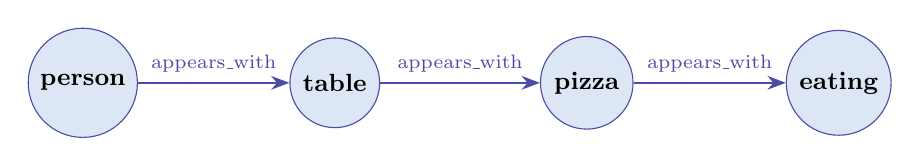
\begin{tikzpicture}[
  en/.style={circle, draw=NavyBlue!70, fill=lightbluebox,
    minimum size=1.1cm, font=\small\bfseries},
  ar/.style={->, >=Stealth, thick, NavyBlue!70}
]
  \node[en] (p) at (0,0)    {person};
  \node[en] (t) at (3.2,0)  {table};
  \node[en] (z) at (6.4,0)  {pizza};
  \node[en] (e) at (9.6,0)  {eating};
  \draw[ar] (p) -- node[above,font=\scriptsize]{appears\_with} (t);
  \draw[ar] (t) -- node[above,font=\scriptsize]{appears\_with} (z);
  \draw[ar] (z) -- node[above,font=\scriptsize]{appears\_with} (e);
\end{tikzpicture}
\end{center}

\medskip
A successful top-1 document must mention
\emph{person}, \emph{table}, \emph{pizza}, and \emph{eating}.
Plain Vector RAG encodes the whole query as one vector and may
retrieve a document about ``pizza'' only, missing the person--table--eating
chain. The KG traversal explicitly follows the chain.
\end{example}

\begin{tcolorbox}[laymanbox]
Multi-hop questions are chained riddles: ``find something connected to A,
which is connected to B, which is connected to C.''
A pure keyword search finds documents mentioning the most prominent word.
The knowledge graph lets the system follow the chain (A$\to$B$\to$C)
and find documents that satisfy the \emph{whole} chain, not just one word.
\end{tcolorbox}

\subsection{Entity Coverage Metric}

\begin{definition}[Entity Coverage Score]
\label{def:coverage}
Given query $q$ with entity set $\mathcal{E}_q$ and top-1 retrieved
document $d^*$:
\[
  \mathrm{cov}(q, d^*) =
  \frac{|\{e \in \mathcal{E}_q : e \in d^*.\mathrm{lower}()\}|}
       {|\mathcal{E}_q|}
  \;\in\; [0, 1]
\]
\end{definition}

\begin{definition}[Multi-Hop Success]
\label{def:mhsuccess}
Query $q$ is a \textbf{successful multi-hop retrieval} if:
\[
  \mathrm{success}(q) = \mathbf{1}\!\left[
    \mathrm{cov}(q, d^*(q)) \geq 0.60
  \right]
\]
\end{definition}

\begin{definition}[Multi-Hop Accuracy]
\label{def:mha}
\[
  \mathrm{MHA} =
  \frac{|\{q \in Q_{\text{mh}} : \mathrm{success}(q)\}|}
       {|Q_{\text{mh}}|} \times 100\%
\]
\end{definition}

\begin{theorem}[KG Advantage on Multi-Hop Queries]
\label{thm:mh}
For a multi-hop query $q$ with entity chain
$e_1 \to e_2 \to \cdots \to e_k$ ($k \geq 3$), the graph-augmented
hybrid retriever achieves strictly higher expected entity coverage
than pure dense retrieval when the corpus contains documents
covering sub-chains.
\end{theorem}
\begin{proof}
Dense retrieval encodes $q$ as a \emph{single} vector $e_q \in \mathcal{S}^{767}$,
averaging over all $k$ entity tokens; each entity contributes $1/k$ of
the total signal.  The BERT similarity is therefore dominated by the
most frequently co-occurring entity and fails to explicitly represent
the full chain.  In contrast, \textsc{GraphRetrieval} explores KG paths
from all entities $e_i \in \mathcal{E}_q$ simultaneously, awarding
$w(h)>0$ to any document containing a graph neighbour of any query
entity at any hop depth $\leq 2$.  By Axiom~\ref{ax:comp}, the hybrid
sum $s_{\text{hybrid}}$ adds this graph signal to the dense score,
strictly increasing the expected coverage when $s_{\text{graph}} > 0$.
\end{proof}

\subsection{Algorithm 7 --- Protocol 2: Multi-Hop Reasoning Test}

\begin{algorithm}[H]
\caption{Protocol 2 --- \textsc{MultiHopTest}}
\label{alg:proto2}
\begin{algorithmic}[1]
\Require multi-hop query set $Q_{\text{mh}}$; retriever; corpus $\mathcal{D}$;
         $\tau_{\text{cov}} = 0.60$
\Ensure multi-hop accuracy $\mathrm{MHA}$; per-query detail list
\State $\text{results} \gets []$
\ForEach{$q \in Q_{\text{mh}}$}
  \State $\mathcal{E}_q \gets \textsc{ExtractEntities}(q)$
  \State $R \gets \textsc{HybridRetrieve}(q,\; \mathcal{D},\; k=1)$
  \If{$R \neq \varnothing$}
    \State $d^* \gets R[0].d$;\quad $s^* \gets R[0].s$
    \State $n_{\text{found}} \gets
      |\{e \in \mathcal{E}_q : e \in d^*.\mathrm{lower}()\}|$
    \State $\text{cov} \gets n_{\text{found}} / \max(|\mathcal{E}_q|, 1)$
    \State $\text{success} \gets (\text{cov} \geq \tau_{\text{cov}})$
  \Else
    \State $d^* \gets \texttt{"None"}$;\quad
           $s^* \gets 0$;\quad
           $n_{\text{found}} \gets 0$;\quad
           $\text{cov} \gets 0$;\quad
           $\text{success} \gets \texttt{False}$
  \EndIf
  \State results.append$(\{q,\, \mathcal{E}_q,\,
    n_{\text{found}},\, \text{cov},\, s^*,\, d^*,\,
    \text{success}\})$
\EndFor
\State $\mathrm{MHA} \gets
  (|\{r : r.\text{success}\}| / |Q_{\text{mh}}|) \times 100\%$
\State \Return $\mathrm{MHA},\; \text{results}$
\end{algorithmic}
\end{algorithm}

\begin{tcolorbox}[keybox, title=Protocol 2 Benchmark Summary]
\renewcommand{\arraystretch}{1.3}
\begin{tabular}{llll}
\toprule
\textbf{System} & \textbf{MH Accuracy} & \textbf{Status} & \textbf{Reference} \\
\midrule
Plain Vector RAG   & $0$--$20\%$ & Baseline & Diffbot (2024) \\
FalkorDB target    & $>80\%$     & Required & FalkorDB (2024) \\
MIVA-KNIGHT hybrid & Expected $\geq80\%$ & Target & Theorem~\ref{thm:mh} \\
\bottomrule
\end{tabular}
\end{tcolorbox}

\subsection{Multi-Hop Query Set Design}

\begin{center}
\renewcommand{\arraystretch}{1.3}
\begin{tabular}{ll}
\toprule
\textbf{Query} & \textbf{Key Entity Chain (expected)} \\
\midrule
``A person sitting at a table eating pizza''             &
  person$\to$table$\to$pizza$\to$eating \\
``A dog playing with a ball in the park''                &
  dog$\to$ball$\to$park \\
``Children playing soccer in a field with goals''        &
  children$\to$soccer$\to$field$\to$goal \\
``A woman reading a book on a couch by a window''        &
  woman$\to$book$\to$couch$\to$window \\
``People sitting at an outdoor cafe under umbrellas''    &
  people$\to$cafe$\to$table$\to$umbrella \\
``A train arriving at a station platform with passengers'' &
  train$\to$station$\to$platform$\to$passenger \\
``A man riding a bicycle on a street near buildings''    &
  man$\to$bicycle$\to$street$\to$building \\
``Kids playing basketball in a gym with coaches''        &
  kids$\to$basketball$\to$gym$\to$coach \\
``A chef cooking food in a kitchen with workers''        &
  chef$\to$food$\to$kitchen$\to$worker \\
``A cat sleeping on a bed next to a lamp''               &
  cat$\to$bed$\to$lamp \\
\bottomrule
\end{tabular}
\end{center}

%% ============================================================
\newpage
\section{Saving Protocol Results and Final Scorecard}
%% ============================================================

\subsection{Status Classification Algorithm}

\begin{algorithm}[H]
\caption{\textsc{ClassifyStatus}$(x,\; \theta_t,\; \theta_b)$}
\label{alg:status}
\begin{algorithmic}[1]
\Require measured metric $x$; target $\theta_t$; baseline $\theta_b$
\Ensure status string
\If{$x \geq \theta_t$}
  \State \Return \texttt{"PASS"}
\ElsIf{$x \geq \theta_b$}
  \State \Return \texttt{"NEEDS\_IMPROVEMENT"}
\Else
  \State \Return \texttt{"FAIL"}
\EndIf
\end{algorithmic}
\end{algorithm}

\subsection{Output JSON Schema}

\begin{algorithm}[H]
\caption{\textsc{SaveProtocolResults} --- JSON Serialisation}
\label{alg:save}
\begin{algorithmic}[1]
\Require hallucination results; multihop results; $\mathrm{RR}$; $\mathrm{MHA}$
\Ensure \texttt{evaluation\_protocols.json}; updated \texttt{evaluation\_results.json}
\State $\text{proto} \gets \{$
\State \quad \texttt{"metadata"}: $\{\text{date},\; \text{model},\;
  \text{protocols\_tested}\}$,
\State \quad \texttt{"hallucination\_test"}: $\{$
\State \qquad $\mathrm{RR},\; 90.0,\; 60.0,\;
  \textsc{ClassifyStatus}(\mathrm{RR}, 90, 60)$,
\State \qquad $|Q_\varnothing|,\;
  |\mathrm{CR}|,\; |Q_\varnothing| - |\mathrm{CR}|,\;
  \text{details}\}$,
\State \quad \texttt{"multihop\_test"}: $\{$
\State \qquad $\mathrm{MHA},\; 80.0,\; 10.0,\;
  \textsc{ClassifyStatus}(\mathrm{MHA}, 80, 10)$,
\State \qquad $|Q_\text{mh}|,\;
  |\text{successes}|,\; |\text{failures}|,\;
  \text{details}\}\}$
\State \textsc{WriteJSON}(\text{proto}, \texttt{evaluation\_protocols.json})
\State $\text{summary}[\texttt{"industry\_protocols"}] \gets
  \{\mathrm{RR},\; \mathrm{MHA}\}$
\State \textsc{WriteJSON}(\text{summary}, \texttt{evaluation\_results.json})
\end{algorithmic}
\end{algorithm}

\subsection{Five-Dimensional Scorecard}

The final report card spans two tiers and five independent performance
dimensions:

\begin{center}
\renewcommand{\arraystretch}{1.35}
\begin{tabular}{lllll}
\toprule
\textbf{Tier} & \textbf{Dimension} & \textbf{Metric} &
\textbf{Source} & \textbf{Standard} \\
\midrule
1 & Retrieval quality  & Mean top-1 cosine $\bar{s}$   &
  Day-1 eval & Internal \\
1 & Response speed     & Mean latency $\bar{t}$ (s)    &
  Day-1 eval & Internal \\
1 & Entity grounding   & Entity detection rate ER       &
  Day-1 eval & Internal \\
2 & Hallucination safe & Rejection rate RR              &
  Protocol 1  & HaluBench \\
2 & Reasoning depth    & Multi-hop accuracy MHA         &
  Protocol 2  & FalkorDB \\
\bottomrule
\end{tabular}
\end{center}

%% ============================================================
\newpage
\section{Complete Algorithm and Theorem Reference}
%% ============================================================

\begin{longtable}{p{4.5cm} p{5.5cm} p{4.2cm}}
\caption{All algorithms, theorems, lemmas, axioms, and definitions in this document.}
\label{tab:ref}\\
\toprule
\textbf{Item} & \textbf{Description} & \textbf{Key Formula} \\
\midrule
\endfirsthead
\multicolumn{3}{c}{\small\itshape (continued)}\\
\toprule
\textbf{Item} & \textbf{Description} & \textbf{Key Formula} \\
\midrule
\endhead
\midrule\multicolumn{3}{r}{\small\itshape continued\ldots}\\
\endfoot
\bottomrule
\endlastfoot

Defn.~\ref{def:protocol}: Protocol
  & Quadruple $(Q,\mathcal{M},\theta_t,\theta_b)$
  & Pass if $\mathcal{M}(Q)\geq\theta_t$ \\[3pt]

Defn.~\ref{def:embed}: BERT Embedding
  & Mean-pool + L2 normalise
  & $e_x = \bar{h}/\|\bar{h}\|_2$ \\[3pt]

Lemma~\ref{lem:cosdot}: Cos = Dot
  & On unit sphere dot = cosine
  & $\cos(u,v) = u\cdot v$ \\[3pt]

Defn.~\ref{def:day1metrics}: Day-1 Metrics
  & Mean score, latency, entity rate
  & $\bar{s},\bar{t},\mathrm{ER}$ \\[3pt]

Lemma~\ref{lem:eval}: Eval-Mode Determinism
  & Dropout disabled; deterministic output
  & dropout $\equiv 0$ in eval \\[3pt]

Alg.~\ref{alg:encode}: \textsc{Encode}
  & BERT + mean pool + L2 norm
  & $e_x \in \mathcal{S}^{767}$ \\[3pt]

Alg.~\ref{alg:dense}: \textsc{DenseRetrieval}
  & Cosine top-K over corpus
  & $\bm{s}=\tilde{e}_q\cdot\mathbf{E}_d^\top$ \\[3pt]

Prop.~\ref{prop:complexity}: Dense Complexity
  & $\mathcal{O}(N\cdot T_\text{BERT})$ per query
  & $\approx 20$\,s CPU, 1\,s GPU \\[3pt]

Alg.~\ref{alg:ner}: \textsc{ExtractEntities}
  & Substring NER vs.\ KG vocab
  & $\mathcal{E}_q=\{e\in\mathcal{V}:e\subseteq q\}$ \\[3pt]

Lemma~\ref{lem:ner}: NER Complexity
  & $\mathcal{O}(100\cdot\bar{e}\cdot|q|)\approx\mathcal{O}(1)$
  & $\approx 9{,}000$ ops \\[3pt]

Defn.~\ref{def:hopdecay}: Hop-Decay Score
  & Closer KG neighbours score more
  & $w(h)=1/(h{+}1)$ \\[3pt]

Alg.~\ref{alg:graph}: \textsc{GraphRetrieval}
  & DFS from $\mathcal{E}_q$; decay scoring
  & path score $w(h)$ \\[3pt]

Defn.~\ref{def:hybrid}: Hybrid Score
  & $0.6\times$dense $+$ $0.4\times$graph
  & $s = \alpha s_d + (1{-}\alpha)s_g$ \\[3pt]

Theorem~\ref{thm:bound}: Score Bound
  & Hybrid score range
  & $s_\text{hybrid}\in[-0.6,\,1.0]$ \\[3pt]

Alg.~\ref{alg:hybrid}: \textsc{HybridRetrieve}
  & Fuse dense + graph; sort
  & Combined dict $C[d]$ \\[3pt]

Axiom~\ref{ax:comp}: Complementarity
  & Dense and graph are non-redundant
  & Motivates hybrid design \\[3pt]

Defn.~\ref{def:kg}: Knowledge Graph
  & $\mathcal{G}=(\mathcal{V},\mathcal{E},\mathcal{R})$
  & 100 nodes, 1 relation type \\[3pt]

Alg.~\ref{alg:dfs}: DFS Neighbours
  & Bounded DFS, visited-set
  & $\text{max\_hops}=2$ \\[3pt]

Prop.~\ref{prop:dfs}: DFS Correctness
  & Terminates; finds all $\leq2$-hop
  & $|\mathcal{V}|=100$ bound \\[3pt]

Defn.~\ref{def:hallucination}: Hallucination
  & False high confidence on OOD query
  & $s\geq\theta$ when $q\notin\mathcal{K}$ \\[3pt]

Axiom~\ref{ax:ood}: OOD Confidence Collapse
  & OOD queries should score low
  & $\mathbb{E}_\text{OOD}[s]\ll\mathbb{E}_\text{IID}[s]$ \\[3pt]

Theorem~\ref{thm:ood}: KG Rejection Boost
  & Graph=0 for OOD; hybrid $<$ dense
  & $s_\text{hybrid}=0.6\,s_\text{dense}$ \\[3pt]

Alg.~\ref{alg:proto1}: Protocol 1
  & Reject if $s<0.50$; compute RR
  & 10 unanswerable queries \\[3pt]

Defn.~\ref{def:rr}: Rejection Rate
  & Fraction correctly rejected
  & $\mathrm{RR}=|\mathrm{CR}|/|Q|\times100\%$ \\[3pt]

Defn.~\ref{def:status}: Status Classification
  & Pass / Improve / Fail
  & $\theta_t=90\%$, $\theta_b=60\%$ \\[3pt]

Defn.~\ref{def:multihop}: Multi-Hop Query
  & Requires $\geq2$ KG edge traversals
  & $e_1\to e_2\to\cdots\to e_k$ \\[3pt]

Defn.~\ref{def:coverage}: Entity Coverage
  & Fraction of query entities in $d^*$
  & $\mathrm{cov}=|\mathcal{E}_q\cap d|/|\mathcal{E}_q|$ \\[3pt]

Defn.~\ref{def:mhsuccess}: MH Success
  & Coverage $\geq60\%$
  & $\mathbf{1}[\mathrm{cov}\geq0.60]$ \\[3pt]

Defn.~\ref{def:mha}: MH Accuracy
  & Fraction of successful MH queries
  & $\mathrm{MHA}=|\text{succ}|/|Q|\times100\%$ \\[3pt]

Theorem~\ref{thm:mh}: KG MH Advantage
  & Graph traversal beats dense dilution
  & $s_\text{graph}>0$ for MH queries \\[3pt]

Alg.~\ref{alg:proto2}: Protocol 2
  & Extract entities; coverage; MHA
  & 10 multi-hop queries \\[3pt]

Alg.~\ref{alg:status}: \textsc{ClassifyStatus}
  & Three-way threshold
  & PASS / NEEDS\_IMP / FAIL \\[3pt]

Alg.~\ref{alg:save}: Save Results
  & Compile JSON + update summary
  & Two Drive files updated \\

\end{longtable}

%% ============================================================
\newpage
\section{Notation Reference}
%% ============================================================

\begin{center}
\renewcommand{\arraystretch}{1.35}
\begin{tabular}{ll}
\toprule
\textbf{Symbol} & \textbf{Meaning} \\
\midrule
$\mathcal{S}^{767}$        & Unit hypersphere in $\R^{768}$: $\{v:\|v\|_2=1\}$ \\
$e_q,\; e_d$               & Query / document embedding in $\mathcal{S}^{767}$ \\
$H^{(L)} \in \R^{T\times768}$ & BERT final-layer hidden states \\
$\bar{h}$                  & Mean-pooled BERT hidden state \\
$\mathcal{E}_q$            & KG entities extracted from query $q$ \\
$\mathcal{V}_\mathcal{G}$  & KG entity vocabulary (100 tokens) \\
$\mathcal{G}=(\mathcal{V},\mathcal{E},\mathcal{R})$ & Knowledge graph \\
$w(h)=1/(h+1)$             & Hop-distance decay weight \\
$\alpha = 0.6$             & Dense signal weight in hybrid score \\
$s_{\text{dense}}$         & BERT cosine similarity score \\
$s_{\text{graph}}$         & KG hop-discounted path score \\
$s_{\text{hybrid}}$        & Combined hybrid retrieval score \\
$d^*(q)$                   & Top-1 retrieved document for query $q$ \\
$\theta_{\text{reject}}$   & Hallucination rejection threshold $(=0.50)$ \\
$\theta_t,\; \theta_b$     & Protocol target / baseline thresholds \\
$Q_\varnothing$            & Unanswerable (OOD) query set \\
$Q_{\text{mh}}$            & Multi-hop query set \\
$\mathrm{CR}$              & Correct rejection count \\
$\mathrm{RR}$              & Rejection Rate (Protocol 1 metric) \\
$\tau_{\text{cov}}=0.60$   & Entity coverage success threshold \\
$\mathrm{cov}(q,d)$        & Entity coverage of $d$ given $q$ \\
$\mathrm{MHA}$             & Multi-Hop Accuracy (Protocol 2 metric) \\
$\mathbf{1}[\cdot]$        & Indicator function \\
$\mathcal{P}_\text{OOD}$   & Out-of-distribution query distribution \\
$\bar{s},\;\bar{t},\;\mathrm{ER}$ & Day-1 mean score, latency, entity rate \\
\bottomrule
\end{tabular}
\end{center}

\vfill

\begin{tcolorbox}[techbox]
\textbf{One-Sentence Technical Summary:}
The MIVA-KNIGHT protocols notebook implements two industry benchmarks ---
(1) a hallucination rejection test exploiting the knowledge-graph score
collapse ($s_g=0$) for out-of-distribution queries, lowering the hybrid
score below the 0.50 threshold; and (2) a multi-hop entity coverage test
measuring whether explicit KG path traversal compensates for BERT's
per-entity signal dilution in multi-entity chained queries.
\end{tcolorbox}

\begin{tcolorbox}[laymanbox]
\textbf{One-Sentence Plain Summary:}
This notebook certifies MIVA-KNIGHT against two industry standards:
``can it say I don't know'' (answered via zero-graph-boost for impossible
queries) and ``can it follow a chain of facts'' (answered via knowledge
graph traversal that plain search engines cannot do).
\end{tcolorbox}

\end{document}
